% a tikz figure for visual processing pipeline

\usetikzlibrary{shapes}

\tikzstyle{data}=[draw,thick,rounded corners,minimum height=1.5cm,text width=2cm,align=center]
\tikzstyle{process}=[rectangle,draw,thick,minimum height=1.5cm,text width=2cm,align=center]

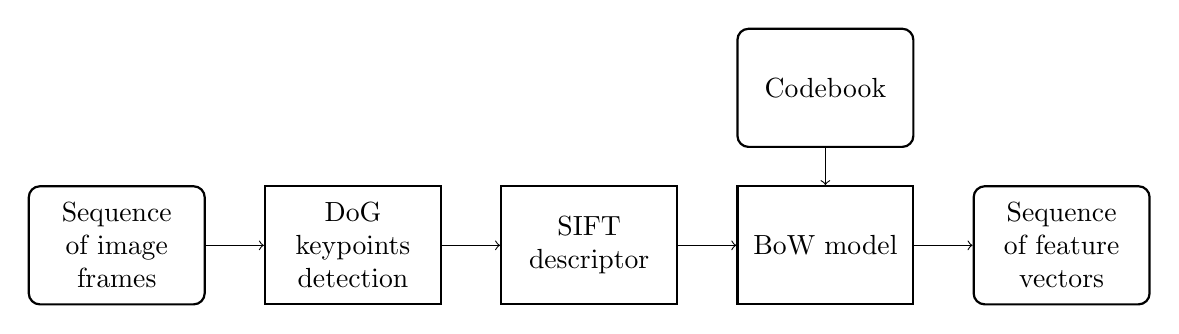
\begin{tikzpicture}[]
  \node[data] (i) at (0,0) {Sequence of image frames};
  \node[process] (p1) at (3,0) {DoG keypoints detection}
    edge [<-] (i);
  \node[process] (p2) at (6,0) {SIFT descriptor}
    edge [<-] (p1);
  \node[process] (p3) at (9,0) {BoW model}
    edge [<-] (p2);
  \node[data] (o) at (12,0) {Sequence of feature vectors}
    edge [<-] (p3);
  \node[data] (o) at (9,2) {Codebook}
    edge [->] (p3);
\end{tikzpicture}

